\section{System requirements}
Anathema is rather tame when it comes to the hardware involved. It has successfully been run on systems featuring a 1.6 GHz CPU with as little as 256 MB of main memory. 20 MB of hard drive space should be more than enough to manage several campaigns of decent size.

While the program does not demand anything special in terms of hardware, there is some software that is required to run the program or at least necessary to make the most out of it.

First of all, Java. Anathema is written in the Java programming language and thus needs a working installation of the Java Runtime Environment to run. The minimum Java version required is version 5.0.

If you are already using Java, you can find out what version you are running by opening a console window and typing \texttt{java --version} followed by the \textsc{Enter} key. The resulting output should look something like this:
\medskip

\small
\texttt{java version "1.5.0\_06"
\newline
Java(TM) 2 Runtime Environment, Standard Edition (build 1.5.0\_06-b05)
\newline
Java HotSpot(TM) Client VM (build 1.5.0\_06-b05, mixed mode)}
\medskip

\normalsize
The version in this case, repeated in each line, is ``1.5.0\_06''. The relevant digit in our case is the second one: If it is 5 or greater, you're fine.

If it reads lower than 5 or if you do not yet have a copy of the Java Runtime Environment installed, point your web browser to the Java website\footnote{http://java.com/en/download/manual.jsp}, where you can always download the latest version for free.
\medskip

In addition to Java, you might want a copy of Adobe Reader to view the documents produced. You can get it free of charge from Adobe\footnote{http://www.adobe.com/products/acrobat/readstep2.html}. Of course, any other program capable of displaying PDF files will suffice.

Finally, for greater enjoyment of the music library features, you will need an audio player capable of handling M3U-Playlists ( such as Winamp or XMMS).
\medskip

Now, with all of that behind us, let's get to the program itself.


\section{Which file to download?}
To download the latest version of Anathema, direct your browser to the Anathema project page\footnote{http://sf.net/projects/anathema} and click the ``Download Anathema'' image displayed. Next, look for the list of ``Latest File Releases'' and locate the entry for package \textsc{anathema} within. Click the link in the ``release'' column, and a screen with all files for the latest release will open.

Mission accomplished? Great.

Know now that within each package are at two flavours of Anathema: A .zip archive suitable for any operating system and more specialized files with their target system clearly indicated. Both kinds contain everything you need to run Anathema, that is the program itself and a flock of supportive files. 

To continue, simply choose the package most appropriate for your operating system, and your download will start. While it is running, you could read on to familiarize yourself with the steps ahead or maybe have a look at our web site to learn about current proceedings.
\medskip

Once the download is finished, you are ready to proceed with the installation.

\section{Installation}
This step is really simple. Just unzip all the files within to an empty directory, using your favorite archive manager. Make sure that all relative path names are kept, lest Anathema misses some files.

Some OS-specific versions feature automated installers to help you along the process.
\medskip

Let's continue the exploration by starting the program.

\section{Launching Anathema}
There are several ways of starting the program, again depending on your operating system.

On most systems you can launch Anathema by opening a console window, changing to the Anathema directory and typing \texttt{java --jar anathema.jar}, followed by a stroke of \textsc{Enter}.

\paragraph{Windows} users may opt to use the executable file anathema.exe that comes with the archive or type \texttt{javaw --jar anathema.jar} instead, but this will swallow any error reports that might come up during launch. Also, a freshly installed Java is configured to launch .jar files when they are double clicked in Windows.

\paragraph{Linux} systems are provided with a shell script, anathema.sh. This configures Anathema to save data in a hidden directory within your home folder and override any settings within the program. See ``Command Line Options'' below for more info on how to customize this script.

\paragraph{Mac OS X} integrates Anathema into it's launcher via the .dmg file provided. Launch it by clicking the icon.
  
\subsection{Command Line Options}
To submit any optional command line parameter to the launcher, you can put \linebreak
\texttt{-D\emph{[Name\_of\_Option]}} between \texttt{java} and the final argument \texttt{-jar anathema.jar}. Currently, this is only used to supply a custom repository directory.

\begin{description}
\item[repository] - Specifies the directory to use for storage and retrieval. If the directory given does not exist, it will be created if necessary read/write--permissions are granted. If the parameter is omitted, a subdirectory ``Repository'' in the main Anathema folder is assumed to be the repository directory.

	Example:\newline
	\texttt{java -Drepository="C:$\backslash$AnathemaRepository" -jar anathema.jar} will instruct Anathema to store and retrieve data from the directory 
	\linebreak``C:$\backslash$AnathemaRepository''.
	
For future launches, a more permanent way of setting the repository directory is provided. We'll address that in a minute.
\end{description}

\begin{figure}[htb]
	\centering
		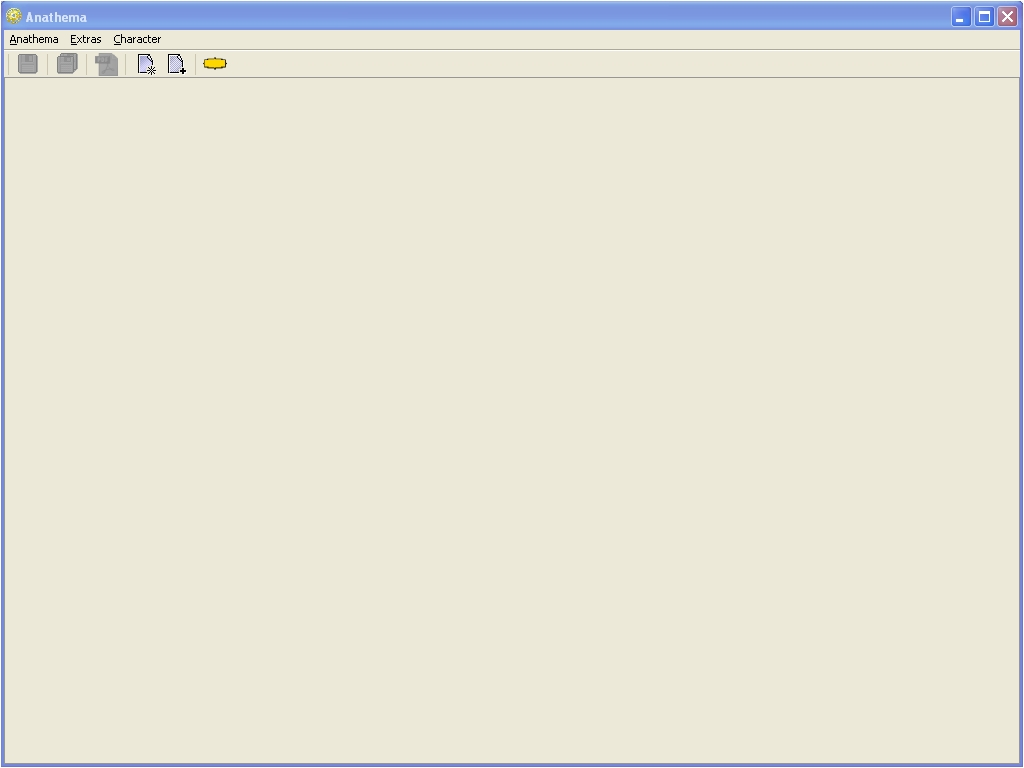
\includegraphics[width=1.00\textwidth]{Images/MainWindow.jpg}
	\caption{The Main Window, Windows Look \& Feel}
	\label{fig:MainWindow}
\end{figure}

\subsection{Done!}
Regardless of the option you chose, Anathema will now load. After a momentary wait, the splash screen will appear, shortly after to be replaced by the main window. The window on screen should now look similiar to figure \ref{fig:MainWindow}.

\paragraph{Congratulations!} Anathema is now ready to use. Go ahead, fool around! Enter all your favourite characters! Create a new one while you're at it!
\medskip

Once you're a tad more familiar with the program, come back here and learn about the various settings in the following section.

\section{Setting your Preferences}\label{sec:Preferences}
Tucked away in the menu \emph{Extras} is an entry called \emph{Preferences}. Clicking there unveils a dialog with - who would have thought - various options for Anathema's basic system. The options are stored on a per-user basis, so every account on your system can have it's own settings. Let's have a closer look:
\begin{description}
	\item[Use Metal Look \& Feel] - Available on Windows systems only. Checking the box forces Anathema to use the ``Metal Ocean'' controls instead of the more Windows-like ones used by default.
	\item[Launch maximized] - The Anathema window is maximized at launch. Useful on resolutions of 1024x768, where part of the window might be hidden by operating system controls at the screen's top and bottom. This option might fail on certain Linux configurations.
	\item[Display document after print] - Controls whether PDF documents are opened in your system's default PDF viewer once printing is done.
	\item[Languange] - Selects the language to run the program in. Currently, English and Spanish are available.
	\item[Show tooltips for (seconds)] - This setting, while global, is mainly intended to control the time until displayed Charm details vanish. 
	\item[Repository directory] - The aforementioned option to permanently set the infamous repository directory. Enter a directory or click the browse button for a graphical selection interface. If the directory does not exist, no changes are made to the setting.
\end{description}
	
When everything is set, click \emph{OK} to commit your changes. A dialog will kindly inform you that you need to restart Anathema to see the effects of any changes. You can do so now or at any later point in time. If you clicked \emph{Cancel} instead, the preferences dialog will vanished and all changes are undone.
\medskip
\newline
This concludes the tour of the Anathema setup.

I hope you enjoy the program and stay with us to experience plenty of new versions and features ahead.
\medskip
\newline
Thank you for using Anathema.
